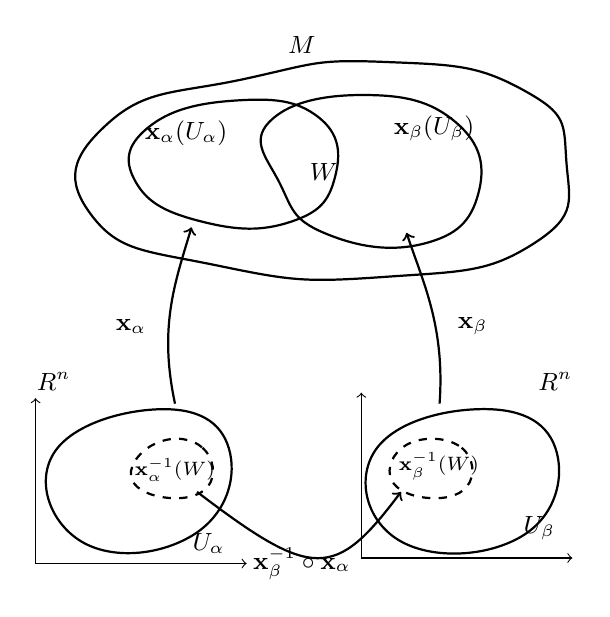
\begin{tikzpicture}[scale=0.7, every node/.style={font=\small}]

    % ---------- Manifold M (top) ----------
    \draw[thick] plot [smooth cycle, tension=0.9] coordinates {
            (-3.5,5.5) (-1,6.3) (1.5,6.6) (4,6.1) (4.8,4.8)
            (4.2,3.3) (1.5,2.7) (-1.5,2.9) (-3.8,3.8)
        };
    \node at (0,6.9) {$M$};

    % region x_alpha(U_alpha)
    \draw[thick] plot [smooth cycle, tension=0.8] coordinates {
            (-2.8,5.4) (-1.2,5.9) (0.3,5.6) (0.6,4.5) (-0.2,3.7) (-1.8,3.7) (-3,4.4)
        };
    \node at (-2.1,5.3) {$\mathbf{x}_\alpha(U_\alpha)$};

    % region x_beta(U_beta)
    \draw[thick] plot [smooth cycle, tension=0.8] coordinates {
            (-0.6,5.5) (1.1,6.0) (2.8,5.5) (3.2,4.2) (2.2,3.3) (0.4,3.5) (-0.4,4.4)
        };
    \node at (2.4,5.4) {$\mathbf{x}_\beta(U_\beta)$};

    % intersection W label
    \node at (0.4,4.6) {$W$};

    % ---------- U_alpha (bottom left) in R^n ----------
    \draw[thick] plot [smooth cycle, tension=0.8] coordinates {
            (-4.5,-0.5) (-2.5,0.3) (-1.3,-0.5) (-2,-2) (-4,-2.1)
        };
    \node at (-1.69,-2.13) {$U_\alpha$};
    \node at (-4.5,0.8) {$\mathbb{R}^n$};

    % preimage of W inside U_alpha
    \draw[thick,dashed] plot [smooth cycle, tension=0.8] coordinates {
            (-2.6,-0.3) (-1.8,-0.4) (-1.7,-1.1) (-2.5,-1.3) (-3.1,-0.9)
        };
    \node (node1) at (-2.3,-0.8) {\scriptsize $\mathbf{x}_\alpha^{-1}(W)$};

    % ---------- U_beta (bottom right) in R^n ----------
    \draw[thick] plot [smooth cycle, tension=0.8] coordinates {
            (1.3,-0.5) (3.2,0.3) (4.6,-0.4) (4,-2) (1.8,-2.1)
        };
    \node at (4.31,-1.86) {$U_\beta$};
    \node at (4.6,0.8) {$\mathbb{R}^n$};

    % preimage of W inside U_beta
    \draw[thick,dashed] plot [smooth cycle, tension=0.8] coordinates {
            (2.0,-0.3) (2.9,-0.4) (3.0,-1.1) (2.2,-1.3) (1.6,-0.9)
        };
    \node at (2.49,-0.74) {\scriptsize $\mathbf{x}_\beta^{-1}(W)$};

    % ---------- Arrows x_alpha, x_beta into M ----------
    \draw[->,thick] (-2.3,0.4) .. controls (-2.6,1.8) and (-2.3,2.6) .. (-2.0,3.6);
    \node at (-3.1,1.8) {$\mathbf{x}_\alpha$};

    \draw[->,thick] (2.5,0.4) .. controls (2.6,1.8) and (2.2,2.6) .. (1.9,3.5);
    \node at (3.1,1.8) {$\mathbf{x}_\beta$};

    % ---------- Transition map arrow between U_alpha and U_beta ----------
    \draw[->,thick] (-1.9,-1.2) .. controls (0.2,-2.8) and (0.6,-2.8) .. (1.8,-1.2);
    \node at (0,-2.5) {$\mathbf{x}_\beta^{-1}\circ \mathbf{x}_\alpha$};

    \draw[->] (-4.83,-2.5) -- (-4.83,0.5);
    \draw[->] (-4.84,-2.5) -- (-1,-2.5);

    \draw[->] (1.08,-2.4) -- (1.08,0.6);
    \draw[->] (1.07,-2.4) -- (4.91,-2.4);
\end{tikzpicture}